\documentclass{article}

\usepackage[utf8]{inputenc}
\usepackage{geometry}
\usepackage{amsmath}
\usepackage{amssymb}
\usepackage{graphicx}
\usepackage{siunitx}
\usepackage{bm}
\usepackage{subfig}

\geometry
{
 a4paper,
 total={170mm,257mm},
 left=20mm,
 top=20mm,
}

\title{Chaos and the N-body Problem}
\author{Michael Hoon Yong Hau \\ 1006617}


\begin{document}

\maketitle

\tableofcontents

\newpage

\section{Introduction}
The theory of dynamical systems was born in the framework of orbital mechanics, through the fundamental work of Poincare and many others, which subsequently has numerous applications in pure and applied research. In Orbital Mechanics, the n-body problem is the problem of predicting the individual motions of a group of celestial objects interacting with each other gravitationally. Solving this problem has been motivated by the desire to understand the motions of the Sun, Moon, planets, and visible stars. The numerical solution to the N-body problem is commonly and inherently chaotic, as we shall see below. \\

\subsection{History of the N-body Problem}
The N-body problem is one of the oldest and most fruitful unsolved problem in the history of science. We shall first understand the simplest case of the N-body problem: the two body problem. The two body problem consists of determining the paths of two gravitationally interacting bodies of known masses and initial velocities. The bodies are moving in three dimensional space and are affected by no other forces than the gravitational forces between them. The first solution of the two-body problem was published by Isaac Newton in 1687 in his work \textit{Principia Mathematica}, along with Johannes Kepler's proof of elliptical orbits in the seventeenth century. 

\subsubsection{Newton's Solution to the Two Body Problem}
The complete two-body problem can be solved by re-formatting it as two one-body problems: a trivial one and one that involves solving for the motion of one particle in an external potential. Newton's proof involved the use of Kepler's Laws and the study of conic sections, specifically elliptical orbits. A modern solution to the problem however, involves the application of differential equations to find the paths for the bodies, which is derived from Newton's Law of Gravitation: 

\begin{equation}
    \textbf{F} = -\frac{Gm_1m_2}{r^2}\frac{\mathbf{r}}{r}
\end{equation} \\

\noindent By Newton's Third Law, each mass experiences this force due to the other masses, this gives:

\begin{equation}
    m_1\mathbf{\Ddot{r}_1} = -\frac{Gm_1m_2}{\lvert\mathbf{r}_2 - \mathbf{r}_1\rvert^3}(\mathbf{r_1}-\mathbf{r_2})
\end{equation}

\begin{equation}
    m_2\mathbf{\Ddot{r}_2} = -\frac{Gm_1m_2}{\lvert\mathbf{r}_2 - \mathbf{r}_1\rvert^3}(\mathbf{r_2}-\mathbf{r_1})
\end{equation} \\

\noindent Solving the differential equations describing the two body problem analytically is trivial. 

\section{The Three Body Problem}
Similarly, Newton treated the three body problem in \textit{Principia Mathematica} to try and understand the Earth-Moon-Sun system, but was unable to find an analytical solution. In 1887, Poincare proved that there is no general analytical closed-form solution, putting an end to all attempts to solve the problem analytically. (There is however, an analytic solution to the \textbf{restricted} three-body diagram, whereby a body of \textbf{negligible} mass moves under the influence of two massive bodies.) Additionally, in the early twentieth century, Einstein developed his theory of general relativity, a geometric model of gravity, which provides additional complications to our three-body problem. \\

\noindent The mathematical statement of the three-body problem can be given in terms of the Newtonian equations of motion for vector positions $\mathbf{r_i} = (x_i, y_i, z_i)$ of three gravitationally interacting bodies with masses $m_i$:

\begin{equation}
    \mathbf{\Ddot{r}_1} = -Gm_2\frac{\mathbf{r_1}-\mathbf{r_2}}{\lvert\mathbf{r_1}-\mathbf{r_2}\rvert^3} - Gm_3\frac{\mathbf{r_1}-\mathbf{r_3}}{\lvert\mathbf{r_1}-\mathbf{r_3}\rvert^3},
\end{equation}

\begin{equation}
    \mathbf{\Ddot{r}_2} = -Gm_3\frac{\mathbf{r_2}-\mathbf{r_3}}{\lvert\mathbf{r_2}-\mathbf{r_3}\rvert^3} - Gm_1\frac{\mathbf{r_2}-\mathbf{r_1}}{\lvert\mathbf{r_2}-\mathbf{r_1}\rvert^3},
\end{equation}

\begin{equation}
    \mathbf{\Ddot{r}_3} = -Gm_1\frac{\mathbf{r_3}-\mathbf{r_1}}{\lvert\mathbf{r_3}-\mathbf{r_1}\rvert^3} - Gm_2\frac{\mathbf{r_3}-\mathbf{r_2}}{\lvert\mathbf{r_3}-\mathbf{r_2}\rvert^3},
\end{equation}

\noindent which is a set of nine second-order differential equations. When modelling a system of 3 bodies interacting gravitationally, the resulting motion is inherently chaotic as can be seen in Figure 1b. \\

\noindent In 1890, Poincare determined that trajectories are commonly aperiodic. However, with the advancement of computer technology in the past few decades, researchers have found more than 600 new families of Newtonian periodic planar collision-less three-body orbits. Examples of these periodic orbits are shown in Figure 1a. \\


\begin{figure}%
    \centering
    \subfloat[\centering Family of Three-body Periodic Orbits]{{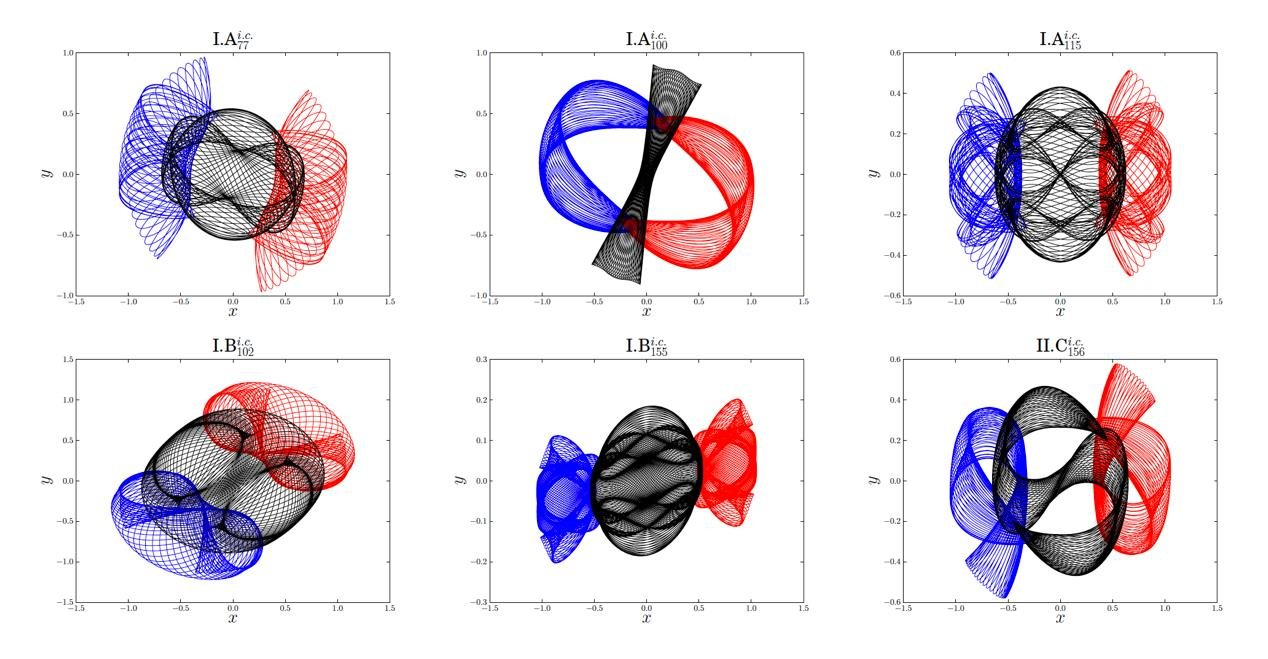
\includegraphics[width=10cm]{Periodic orbits.jpg} }}%
    \qquad
    \subfloat[\centering Chaotic Three Body Interaction]{{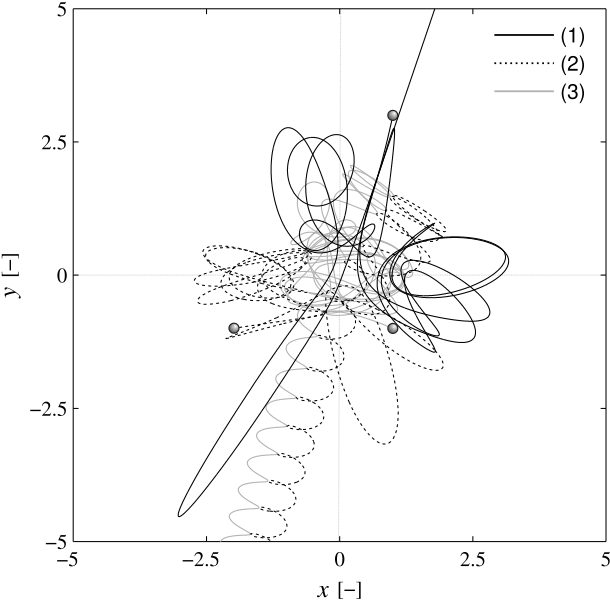
\includegraphics[width=6cm]{three body orbit.png} }}%
    \caption{Orbits of Three Bodies}%
    \label{fig: three body}%
\end{figure}

\section{Chaos in the N-body Problem}
The N-body equations of motion are given by: 

\begin{equation}
    \mathbf{\Ddot{r}_i} = -G \sum_{\substack{j=1 \\ j\neq i}}^N m_j \frac{\mathbf{r_i}-\mathbf{r_j}}{\lvert\mathbf{r_i}-\mathbf{r_j}\rvert^3}
\end{equation} 

\noindent Again, there exists no closed-form solutions to the system of differential equations governing N-body dynamics, and thus solutions must be obtained numerically, via complex algorithms such as LSODA. More recent solutions to the three-body and N-body problems have utilised Deep Neural Networks. However, due to sensitive dependence on initial conditions, the chaotic nature of the three-body problem is still difficult to numerically model even with accurately trained Neural Networks. N-body simulations have also gained in popularity following the development of parallel compute platforms such as NVIDIA CUDA. 

\begin{figure}[h]
    \centering
    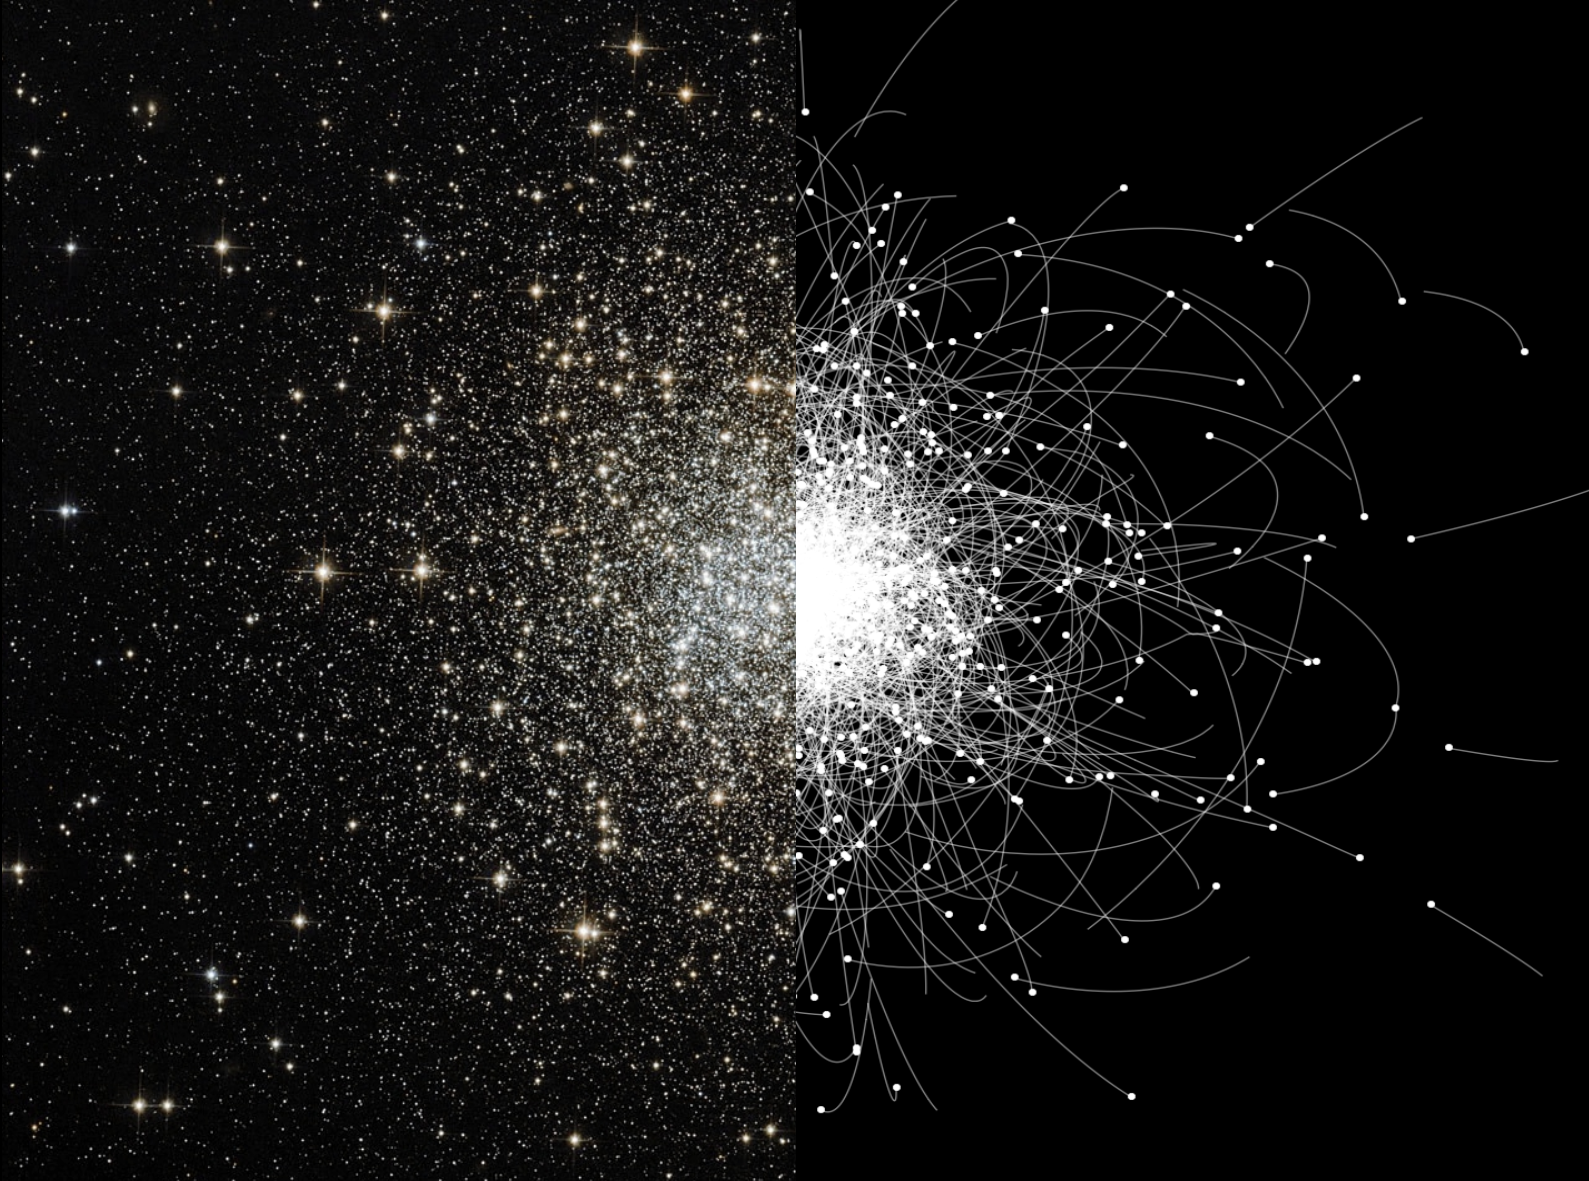
\includegraphics[width=0.55\textwidth]{nbody.png}
    \caption{N-Body Simulation (right) of NGC 7006 Galaxy Cluster, Hubble (left)}
    \label{fig:nbody}
\end{figure}

\section{Other Applications of the N-body Problem}
The N-body problem does not only apply in the case of massive bodies interacting via the gravitational force. 

\subsection{N-body Problem in Machine Learning}
Consider the field of Statistical Deep Learning: there is now an emerging N-body problem in more advanced systems. One common example is the development of Multi-agent Reinforcement Learning, where multiple learning agents coexist in a shared environment. Each agent is motivated by its own rewards, and does actions to advance its own interests; in some environments these interests are opposed to the interests of other agents, resulting in complex group dynamics. This is analogous to our N-body problem above. Multi-agent Reinforcement Learning has many interesting applications in Game Theory and Swarm Robotics, which are currently being studied now. \\

\section{Bibliography}
Image References: \\

\noindent [1a] Li, X., Liao, S. More than six hundred new families of Newtonian periodic planar collisionless three-body orbits. Sci. China Phys. Mech. Astron. 60, 129511 (2017). https://doi.org/10.1007/s11433-017-9078-5 \\

\noindent [1b] Roa, Javier & Urrutxua, Hodei & Pelaez, Jesus. (2016). Stability and chaos in Kustaanheimo-Stiefel space induced by the Hopf fibration. Monthly Notices of the Royal Astronomical Society. 000. 1-12. 10.1093/mnras/stw780. \\

\noindent [2] Dorval, J., et al. “Hubble–Lemaître Fragmentation and the Path to Equilibrium of Merger-Driven Cluster Formation.” Monthly Notices of the Royal Astronomical Society, vol. 459, no. 2, Mar. 2016, pp. 1213–32. Crossref, https://doi.org/10.1093/mnras/stw714.

\end{document}
